%----------------------------------------------------------------
%
%  File    :  survey.tex
%
%  Author  :  Keith Andrews, IICM, TU Graz, Austria
%
%  Created :  24 Mar 2010
%
%  Changed :  06 Dec 2016
%
%----------------------------------------------------------------


\documentclass[11pt,onecolumn,twoside]{report}

\usepackage[          % set page and margin sizes
  a4paper,
  twoside,
  top=5mm,
  bottom=10mm,
  inner=15mm,
  outer=15mm,
  bindingoffset=10mm,
  head=10mm,
  foot=10mm,
  headsep=15mm,
  footskip=15mm,
  includeheadfoot,
]{geometry}
% A4 is 210 x 297 mm



\usepackage{txfonts}            % new times fonts
\usepackage{relsize}            % relative font sizes \smaller \larger
\usepackage{float}              % H for float placement
\usepackage{setspace}           % line spacing

\usepackage[T1]{fontenc}        % 8-bit output chars (must be before inputenx)
\usepackage[utf8]{inputenx}     % input char encoding

\usepackage{textcomp}           % symbols such as \texttimes and \texteuro
\usepackage{latexsym}

\usepackage{xspace}
\usepackage{etoolbox}           % for \newrobustcmd
\usepackage{makecmds}           % for \makecommand


\usepackage[english,austrian,british]{babel}


\usepackage[bf,sf]{titlesec}



\setlength{\textfloatsep}{10mm plus 2mm minus 1mm}
\setlength{\floatsep}{10mm plus 2mm minus 1mm}
\setlength{\intextsep}{10mm plus 2mm minus 1mm}

\setlength{\dbltextfloatsep}{10mm plus 2mm minus 1mm}
\setlength{\dblfloatsep}{10mm plus 2mm minus 1mm}

\setlength{\abovecaptionskip}{4mm plus 2mm minus 1mm}
\setlength{\belowcaptionskip}{0mm}




% use caption and subfig (caption2 and subfigure are now obsolete)

\usepackage[
  position=bottom,
  margin=1cm,
  font=small,
  labelfont={bf,sf},
  format=hang,
  indention=0mm,
]{caption,subfig}

\captionsetup[subfigure]{
  margin=0pt,
  parskip=0pt,
  hangindent=0pt,
  indention=0pt,
  singlelinecheck=true,
}




% fancyhdr to make nice headers and footers
% and deal with long chapter names

\usepackage{fancyhdr}         % headers and footers
\pagestyle{fancy}             % must call to set defaults before redefining

\renewcommand{\chaptermark}[1]{%
  \markboth{\thechapter.\ #1}{}
}
\renewcommand{\sectionmark}[1]{%
  \markright{\thesection.\ #1}
}
\renewcommand{\headrulewidth}{0mm}
\renewcommand{\footrulewidth}{0mm}
\newcommand{\headlook}{\sffamily}
\fancyhf{}
\fancyhead[LE,RO]{\thepage}
\fancyhead[LO]{%
\parbox[t]{0.8\textwidth}{\headlook\nouppercase{\rightmark}}
}
\fancyhead[RE]{%
\parbox[t]{0.8\textwidth}{\raggedleft\headlook\nouppercase{\leftmark}}
}


%\fancypagestyle{plain}{%   redefine plain style, but doesn't work
%  \fancyhf{}    % clear all header and footer fields
%  \fancyfoot[C]{\headlook \thepage} % except the center
%  \renewcommand{\headrulewidth}{0pt}
%  \renewcommand{\footrulewidth}{0pt}
%}



\usepackage{xcolor}
\definecolor{darkgreen}{rgb}{0.0,0.2,0.0}
\definecolor{darkblue}{rgb}{0.0,0.0,0.2}
\definecolor{darkred}{rgb}{0.2,0.0,0.0}
\definecolor{verylightgrey}{gray}{0.95}
\definecolor{lightgrey}{gray}{0.9}
\definecolor{black}{gray}{0.0}


\usepackage{tabularx}


\usepackage{listings}                 % for listings of source code
\usepackage{calc}                     % for calulation below

\makeatletter
\newlength{\numwidth}%
\setlength{\numwidth}{\widthof{\normalfont{\lst@numberstyle{99}}}}% Up to 2-digit (99) line numbers
\def\lst@PlaceNumber{%
  \makebox[\numwidth+1em][l]{%
    \makebox[\numwidth][r]{\normalfont\lst@numberstyle{\thelstnumber}}%
  }%
}
\makeatother

\lstset{                              % set parameters for listings
  floatplacement=tp,                  % default float placement
  numberbychapter,
  inputencoding=utf8,
  language=,                          % empty = plain text
  basicstyle=\small\ttfamily,
  tabsize=2,
  xleftmargin=1cm,
  xrightmargin=1cm,
  frame=none,
  framexleftmargin=0mm,
  rulesepcolor=\color{verylightgrey},
  numbers=none,
  numberstyle=\scriptsize,
  numbersep=2ex,
  breaklines,
  showtabs=false,
  showspaces=false,
  showstringspaces=false,
  keywordstyle=\bfseries,
  identifierstyle=,
  stringstyle=,
  captionpos=b,
  abovecaptionskip=\abovecaptionskip,
  belowcaptionskip=\belowcaptionskip,
  aboveskip=\floatsep,
  belowskip=\floatsep,
  extendedchars=true,
  literate=%
    {©}{{\textcopyright}}1
    {€}{{\texteuro}}1
    {Ö}{{\"O}}1
    {Ä}{{\"A}}1
    {Ü}{{\"U}}1
    {ß}{{\ss}}1
    {ö}{{\"o}}1
    {ä}{{\"a}}1
    {ü}{{\"u}}1,       % map some utf8 chars to replacements
}


\lstdefinelanguage{biblatex}   % based on biblatex v 2.7a from 2013-07-14
{
  keywords={%
    @article,@book,@mvbook,@inbook,@bookinbook,@suppbook,%
    @booklet,@collection,@mvcollection,@incollection,@suppcollection,%
    @manual,@misc,@online,@patent,@periodical,@suppperiodical,%
    @proceedings,@mvproceedings,@inproceedings,@reference,@mvreference,%
    @inreference,@report,@set,@thesis,@unpublished,@xdata,%
    @conference,@electronic,@mastersthesis,@phdthesis,@techreport,@www,%
    @artwork,@audio,@bibnote,@commentary,@image,@jurisdiction,@legislation,%
    @legal,@letter,@movie,@music,@performance,@review,@software,%
    @standard,@video%
  },
  comment=[l][\itshape]{@comment},
  sensitive=false,
}


\usepackage[short]{datetime}   % load datetime *after* babel, requires fmtcount
% \newdateformat{britdate}{%
% \ordinaldate{\THEDAY} \,\monthname[\THEMONTH] \THEYEAR
% }
\newdateformat{keithdate}{%
\twodigit{\THEDAY}~\shortmonthname[\THEMONTH]~\THEYEAR
}


\usepackage[hyphens,obeyspaces]{url}
\def\UrlFont{\smaller\ttfamily}



\usepackage[
  autostyle,
  english=british,
  threshold=0,
  thresholdtype=lines,
]{csquotes}
\renewcommand{\mkcitation}[1]{\space#1}

\newenvironment*{smallquote}          % smaller text within a block quote
  {\quote\smaller}
  {\endquote}
\SetBlockEnvironment{smallquote}

% put quotation marks around block quotes
% \renewenvironment{quoteblock}{\openautoquote}{\closeautoquote}

% I prefer double quotes as outer
\DeclareQuoteStyle[keithbritish]{british}%  [variant]{style}
  {\textquotedblleft}%                      opening outer mark
  {\textquotedblright}%                     closing outer mark
  [0.05em]%
  {\textquoteleft}%                         opening inner mark
  {\textquoteright}%                        closing inner mark

\setquotestyle[keithbritish]{british}



\usepackage[
  backend=biber,
  bibstyle=authoryear-ka,
  citestyle=authoryear-ka,
  sorting=nyt,
  useprefix,                   % van and von are part of second name
  mergedate=false,             % only for authoryear style
  dashed=false,                % only for authoryear style
  abbreviate=false,
  maxcitenames=2,              % if more than two authors, then use et al
  mincitenames=1,              % if exceeds 2 authors, then use 2
  maxbibnames=99,              % print all authors in biblio
  uniquename=init,
  hyperref=true,
  backref=true,
  backrefstyle=two,
  natbib=true,
  sortlocale=en,
]{biblatex}



% set for csquotes, but \autocite only available
% after biblatex is loaded
\SetCiteCommand{\autocite}    % or maybe \parencite

% more space between entries in bib
\setlength\bibitemsep{1.5\itemsep}


% remove URL: from in front of URLs
\DeclareFieldFormat{url}{\url{#1}}
\DeclareFieldFormat{doi}{\doi{#1}}
\DeclareFieldFormat{isbn}{\isbn{#1}}
\DeclareFieldFormat{issn}{\issn{#1}}

% suppress urldate field
\DeclareSourcemap{
  \maps[datatype=bibtex]{
    \map{
      \step[fieldset=urldate, null]
    }
  }
}

% for article titles
\DeclareFieldFormat{title:article}{\emph{#1}\midsentence}

\DefineBibliographyStrings{british}{%
  january          = {Jan},
  february         = {Feb},
  march            = {Mar},
  april            = {Apr},
  may              = {May},
  june             = {Jun},
  july             = {Jul},
  august           = {Aug},
  september        = {Sep},
  october          = {Oct},
  november         = {Nov},
  december         = {Dec},
}



% \bibliography{kandrews,latex,writing,inm-plag}

%\addbibresource{writing.bib}
%\addbibresource{latex.bib}
%\addbibresource{kandrews.bib}
%\addbibresource{ivis.bib}
\addbibresource{G5.bib}
\addbibresource{images/imgLocations.bib}
\addbibresource{listings/codeSource.bib}




\usepackage{ifpdf}

\ifpdf
  % pdflatex
  \usepackage[pdftex]{graphicx}
  \DeclareGraphicsExtensions{.pdf,.jpg,.png}
  \pdfcompresslevel=9
  \pdfpageheight=297mm
  \pdfpagewidth=210mm
  \usepackage[         % hyperref should be last package loaded
    unicode,
    pdftex,
    pdftitle={Web UI Animation},
    pdfsubject={},
    pdfauthor={Rok Kogovšek, Alexei Kruglov, Fernando Pulido Ruiz, and Helmut Zöhrer},
    pdfkeywords={survez, IAWEB, animation, UI, web},
    bookmarks,
    bookmarksnumbered,
    linktocpage,
    colorlinks,
    linkcolor=darkred,
    anchorcolor=red,
    citecolor=darkgreen,
    urlcolor=darkblue,
    pdfview={FitH},
    pdfstartview={Fit},
    pdfpagemode=UseOutlines,       % open bookmarks in Acrobat
    plainpages=false,              % avoids duplicate page number problem
    pdfpagelabels,                 % avoids duplicate page number problem
    breaklinks=true,               % allow links exceeding a single line
  ]{hyperref}

\else
  % latex
  % should never have to run latex, since l2h now understands pdflatex .aux
  \usepackage[dvips]{graphicx}
  \usepackage[dvips]{hyperref}
  \DeclareGraphicsExtensions{.eps}
\fi





% \liintro list item intro is a style used when list items have an
% introduction phrase (say in italics) followed by a colon.
\newcommand{\liintro}[1]{\emph{#1}}


\newcommand{\imgcredit}[1]
{\smaller{}[#1]}



\newcommand{\copyrightACM}
{%
Copyright \copyright\ by the Association for Computing Machinery, Inc.%
}




\newcommand{\daymonthyear}[3]
{%
\twodigit{#1}\hspace{0.7ex}\nolinebreak[2]\shortmonthname[#2]\hspace{0.7ex}\nolinebreak[2]#3%
}


\newcommand{\monthyear}[2]
{%
\shortmonthname[#1]\hspace{0.7ex}\nolinebreak[2]#2%
}


\newcommand{\yearmonthday}[3]
{%
\twodigit{#3}\hspace{0.7ex}\nolinebreak[2]\shortmonthname[#2]\hspace{0.7ex}\nolinebreak[2]#1%
}


\newcommand{\yearmonth}[2]
{%
\shortmonthname[#2]\hspace{0.7ex}\nolinebreak[2]#1%
}



% link to Amazon or
% http://worldcatlibraries.org/wcpa/isbn/[ISBN number]

\newrobustcmd{\isbn}[1]
{%
{%
\ifpdf
{\smaller ISBN}
\href{http://www.amazon.com/exec/obidos/ASIN/#1/keithandrewshcic}{#1}%
\else
{\smaller ISBN}
#1%
\fi
}%
}



% ISSN
% http://www.bl.uk/services/bibliographic/issn.html
% 8 digits, should be printed xxxx-xxxx
% e.g. 0020-0190 is Information Processing Letters, Elsevier
%
% Lookup services:
% http://kmittlib.lib.kmutt.ac.th:81/search/i?SEARCH=0020-0190
% http://worldcatlibraries.org/wcpa/issn/0020-0190

\newrobustcmd{\issn}[1]
{%
{%
\ifpdf
{\smaller ISSN}
\href{http://worldcatlibraries.org/wcpa/issn/#1}{#1}%
\else
{\smaller ISSN}
#1%
\fi
}%
}



% DOIs  http://www.doi.org/  e.g.
% doi:10.1038/nature723
% http://dx.doi.org/10.1038/nature723

\newrobustcmd{\doi}[1]
{%
{%
\def\UrlFont{\rmfamily}
\ifpdf                                   % pdflatex
\href{http://dx.doi.org/#1}{doi:\protect\nolinkurl{#1}}%
\else                                    % latex
doi:\protect\nolinkurl{#1}%
\fi
}%
}





\newrobustcmd{\website}[1]
{%
\ifpdf                                  % pdflatex
\href{http://#1/}{\nolinkurl{#1}}%
\else                                   % latex
\nolinkurl{#1}%
\fi
}




\newcommand{\news}[1]
{%
\ifpdf
\href{news:#1}{\nolinkurl{#1}}
\else
\nolinkurl{#1}%
\fi
}








% based on url package
% define styles for class, file, and variable names
% which break nicely at line breaks

% make the macros robust so they work inside captions, etc

\newcommand{\ttname}{\begingroup \smaller\urlstyle{tt}\Url}
\newcommand{\rmname}{\begingroup \smaller\urlstyle{rm}\Url}
\newcommand{\sfname}{\begingroup \smaller\urlstyle{sf}\Url}


% cname is for class names
\newrobustcmd{\cname}[1]{\sfname{#1}}

% fname is for file names and directory names
\newrobustcmd{\fname}[1]{\ttname{#1}}

% vname is for variable names, domain names, email addresses
\newrobustcmd{\vname}[1]{\ttname{#1}}



% Euro symbol
\newcommand{\euro}{\texteuro\,}

% times symbol
\newcommand{\timessym}{\texttimes\,}

% approx symbol
\newcommand{\approxsym}{\ensuremath\approx\,}

% plusminus symbol
\newcommand{\plusminussym}{\textpm\,}

% not equal symbol
\newcommand{\neqsym}{\ensuremath{\neq\,}}

% rightarrow symbol
\newcommand{\rightarrowsym}{\ensuremath\rightarrow\,\,}




\newcommand{\TODO}[1]
{
{\textcolor{red}{[TODO: #1]}}
}



\newcommand{\fullh}{18cm}         % height of figures for 1 per page
\newcommand{\halfh}{9.5cm}        % height of figures for 2 per page
\newcommand{\thirdh}{6cm}         % height of figures for 3 per page


\tolerance=400 
  % makes some lines with lots of white space, but      
  % tends to prevent words from sticking out in the margin





\definecolor{lightgray}{rgb}{.9,.9,.9}
\definecolor{darkgray}{rgb}{.4,.4,.4}
\definecolor{purple}{rgb}{0.65, 0.12, 0.82}
\lstdefinelanguage{JavaScript}{
	keywords={break, case, catch, continue, debugger, default, delete, do, else, false, finally, for, function, if, in, instanceof, new, null, return, switch, this, throw, true, try, typeof, var, void, while, with},
	morecomment=[l]{//},
	morecomment=[s]{/*}{*/},
	morestring=[b]',
	morestring=[b]",
	ndkeywords={class, export, boolean, throw, implements, import, this},
	keywordstyle=\color{blue}\bfseries,
	ndkeywordstyle=\color{darkgray}\bfseries,
	identifierstyle=\color{black},
	commentstyle=\color{purple}\ttfamily,
	stringstyle=\color{red}\ttfamily,
	sensitive=true
}






\lstset{
	backgroundcolor=\color{lightgray},
	float=tp,
	xleftmargin=1cm,
	xrightmargin=1cm,
    framexleftmargin=1mm,
	extendedchars=true,
	basicstyle=\footnotesize\ttfamily,
	showstringspaces=false,
	showspaces=false,
	numbers=left,
	numberstyle=\footnotesize,
	numbersep=9pt,
	tabsize=2,
	breaklines=true,
	showtabs=false,
	captionpos=b
}



\begin{document}

\keithdate

\normalsize
\pagestyle{empty}         % for preliminary pages (no numbers shown)
\pagenumbering{Roman}     % for pdf labels




\begin{titlepage}

\begin{center}
{\Large \sffamily \bfseries Web UI Animation}

\vspace{1cm}

% {\large\sffamily Keith Andrews}

{\large\sffamily Group 5}

\vspace{5mm}

{\large\sffamily Rok Kogovšek, Alexei Kruglov, Fernando Pulido Ruiz, and Helmut Zöhrer}

\vspace{1cm}

% Institute for Information Systems and Computer Media (IICM), \\
% Graz University of Technology \\
% A-8010 Graz, Austria \\[1cm]


{\large
706.041 Information Architecture and Web Usability WS 2016 \\
Graz University of Technology \\
A-8010 Graz, Austria  \\[1cm]
}

\vspace{1cm}

% {\large 22 Nov 2016}

{\large \today}


\end{center}



\vspace{2cm}

\begin{quote}
\begin{center}
{\large\sffamily\bfseries Abstract}
\end{center}

This survey tries to give insights into the uses of web animations and possible ways of creating them with CSS and JavaScript. Not only, why they should be used on a website, but also when to use CSS or JavaScript, will be covered. We also explore the enhancement of animation through SVG. In addition to the theoretical background, numerous practical code examples will be included and discussed. 

\end{quote}

\vfill

\begin{center}
{\small\sffamily \copyright ~ Copyright 2016 by the author(s),
except as otherwise noted.}

\vspace{2mm}
{\footnotesize\sffamily This work is placed under a
Creative Commons Attribution 4.0 International
(\href{https://creativecommons.org/licenses/by/4.0/}{CC BY 4.0}) licence. It uses the LaTex template from "Writing a Survey Paper" by Keith Andrews, used under CC BY 4.0 / Desaturated from original
}
\end{center}

\end{titlepage}




\cleardoublepage
\pagestyle{plain}
\pagenumbering{roman}



{
\setlength{\parskip}{3pt plus 3pt minus 3pt}     % compact tables of contents
\tableofcontents
\addcontentsline{toc}{chapter}{Contents}

\cleardoublepage
\listoffigures
\addcontentsline{toc}{chapter}{List of Figures}

%\cleardoublepage
%\listoftables
%\addcontentsline{toc}{chapter}{List of Tables}

\cleardoublepage
\renewcommand{\lstlistlistingname}{List of Listings}
\lstlistoflistings
\addcontentsline{toc}{chapter}{List of Listings}
}

% define CSS source code coloring
\lstdefinelanguage{CSS} 
{ 
keywords={},
% CSS properties
keywords={ border,transform,transition,duration,timing-function,animation,color,background,margin,padding,font,weight,display,position,top,left,right,bottom,list,style,size,white,space,min,width,opacity},
% CSS rules
keywords=[2]{@keyframes},
% CSS selectors
keywords=[3]{hover,before,after},
sensitive=false, 
morecomment=[l]{//}, 
morecomment=[s]{/*}{*/}, 
morestring=[b]",
keywordstyle=\color{blue},
keywordstyle=[2]\color{violet},
keywordstyle=[3]\color{orange}
}

\cleardoublepage
\pagestyle{headings}        % for main pages
\pagenumbering{arabic}

\cleardoublepage
%----------------------------------------------------------------
%
%  File    :  survey-intro.tex
%
%  Author  :  Keith Andrews, IICM, TU Graz, Austria
% 
%  Created :  27 May 1993
% 
%  Changed :  06 Dec 2016
% 
%----------------------------------------------------------------


\chapter{Introduction}

\label{chap:Intro}

Web animations are not only there to look pretty. Animated objects may carry 
meaning and we will see that there is much more thinking and planning necessary 
than expected at first sight. 

Knowing this makes it difficult to find the right amount of animation without 
overdoing it. Some animation just for the purpose that something happens on the 
screen will not do any good to the user and might lead to distraction. 

The basic way of implementing animations is with Cascading Style Sheets (CSS). 
It is widely supported and offers rather simple but effective ways of 
transforming objects in a meaningful way. Especially keyframes and easing 
effects are widely used for animating objects. 
The explicit implementation of hamburger menus, loading icons and navigation 
bars is described in detail in this survey. 

Similar to CSS, SVG animations are possible as well. They have the feature of 
including basic graphical elements and have the advantage of being infinitely 
scalable which might come handy in the online use. 

Another way of implementing animations is via JavaScript (JS). It allows more 
complex creations and gives the developer much more possibilities and freedom. 
It requires longer loading times and generally takes up more memory than pure 
CSS animations though. A combination of CSS and JS can be useful for a wide 
variety of animation effects. 
Especially the possibilities of animating text with JS and CSS are underlined 
in this survey. 


% Fernando Pulido Ruiz
\cleardoublepage
%----------------------------------------------------------------
%
%  File    :  survey-animation.tex
%
%  Author  :  Fernando Pulido Ruiz, TU Graz, Austria
% 
%  Created :  01 Dec 2016
% 
%  Changed :  X Dec 2016
% 
%----------------------------------------------------------------


\chapter{Animation}

\label{chap:Animation}

{\em"Animation is defined as changing some property over time. On the other hand, motion is the act of moving or the process of being moved. . . .  To put it more simply, all motion is animation, but not all animation is motion."}\citep{head2016designing}

\section{Not Just Motion!} % (fold)
\label{sec:anime_motion}

In animation we change an object’s attribute(s) over time to achieve an objective. As stated by \citet{head2016designing}, animation is much more than adding movement to an object. Movement of an object can be described by a change of its 6 degrees of freedom, them being the coordinates in 3D space and the rotation around the 3D space axises. However an object has usually many more changeable attributes or properties. One could animate color changing and fading, invisibility through transparency, growth with scaling, focus with blurring, etc.

\section{Why Animation in Web UI?} % (fold)
\label{sec:anime_why}

\TODO{Missing: improve decision making, user feedback}

While writing this survey, with so much animation theory, a hilarious idea was just coming up to mind. Have you ever stopped to think about why some people just seem to be more funny than others? And of course, this happens everyday. Just think about a good joke told by someone with no real humour. It is meaningless. Now, think about the same joke being told by a profesional comedian on TV telling jokes over the weekend. Way more funny, is it not? But the point is, why and how is this be possible?
%In some sense, it has to do with \ldots animation. The fact is that we somehow could be thought as animated objects. We move, we produce sound, and we show our feelings through those moves and sounds. Furthermore, our feelings can even be influenced by how those sounds and moves we see are! So, having made this clear, now it can be better understood the reason of prefering one guy or another one telling the same joke.
It has lots to do with how they speak and how they move! As well of other minor factors. That, I am afraid, is the same as with animation. 

Animation, be it in a cartoon, webpage, app or anywhere else, adds a new level of communication which can be hard to explain , but easy to feel. It creates a special connection between what the message is intended to be, and the receiver. It allows an additional cannel of invisible information to exist, and makes the viewer feel part of the process, and gets his attention grabbed in a practical way.

We always need to understand, where we are and where are we going to. Animation can helps us with this and even can improve the use of resources. Just think about when trying to navigate through a small screen. Having some animated window coming out when you put your mouse on, does not only save space (which is already a good enough reason to implement it), but makes the entire process of navigating easier and simpler. A user does not really want to think while navigating, and this can be fulfilled with animation. They can be guided, orientated or helped in going through a process just with animation, which will of course improve their user experience and make them feel more sure and comfortable about what they are doing, without thinking they are in a real puzzle and need to make big use of their brains.

Nowadays, it´s very common to access many sites through different devices. Just think about when trying to know any train timetable. You probably have the app in your Smartphone, but depending on where are you at the moment, you might just google it up and search it through their webpage. Having animation allows sites to connect context and media. A user will just find himself guided throught the process no matter where he is or what device is he using, because of being under some potential animation process. 

But, how do these animations grab people´s atention? There are over twelve basic principles, written by Disney, but two of them are like the foundation of animation, and the rest basically build up from them. Timing and spacing. Timing can be understood as the time length of an action to happen, let’s say the duration of it, while spacing could be explained as the speed changes during one of these actions in an animation. 
\citet{head2016designing} (Chapter 2, page 18) describes their impact with: {\em“Timing and spacing convey the mood, emotion, and reaction of an object.”}

%Both of them act synergistically, transmitting the viewer all of the feelings and advantages listed aboved.

\section{Aim For Invisible Animation} % (fold)
\label{sec:anime_invisible}

In animation, it is very common during the designing process to end up messing things up. As a general rule, as a designer, your one good way to show love to the user is actually not making his or her life harder accomplishing the task at hand. Certainly designers do not hold such ill intentions, but as said before, it is quite easy and happens very often just to have users unnecesarily waiting for an animation to finish or having a hard time finishing a task due to animation. It could be said that the perfect animation is the one which is not noticed. That´s not 100\% accurate, but a good idea in general. 

\vspace{5mm}

{\em“Good interface animations need to be flexible and always feel responsive to a user’s input even if the animation is currently animating.”}\citet{head2016designing} (Chapter 3, page 48)

\vspace{5mm}

Users need feedback to feel themselves listened and understood. Animation can be understood as a bridge which takes the user to a higher quality experience. If an animation doesn’t respect having the user happily informed with feedback, its experience quality will of course drop and so will the trust towards the UI. A user will never feel comfortable in a system which does not take into consideration its input. 

It is also important, that an animation should never be a show-off work. It should be always remembered, that in general, the user interacting with an animation, is probably willing to do or finish something. A UI user is not just laying there waiting for an animation to happen and look at it itself and enjoy it. That could be the aim of animators years ago where they were really telling stories and people were fascinted about it. But times changed, and now the timing requirements are no longer the same as in those days. Study and carefully think about the suitable timing for each animation, because a short amount of milliseconds can be the limit between failing or succeeding. Good timing is more an art than a science \citep{head2016designing}.
%(when talking about a user’s satisfaction, of course). Val Head [2016] smartly points out that good timing is more an art than a science(PARAPHRASING: VAL HEAD’S BOOK, CHAPTER 3, PAGE 52).

\section{Development of animation} % (fold)
\label{sec:anime_dev}

\TODO{Missing part, COPIED JUST THE POINTS FROM SLIDES}

Often problems in development

Usually discussed at the end stages of the project.
Seen just as extra decoration.
Should be part of the design!
When everything is finished, it is "too late" to replan design (animation).
Animation is underestimated in design.

Where to start planning?

Start with planning already in early stages.
Animation can replace a fixed design element.
Add only animation that helps user and does not distract or lowers the UX.
Write about animation also in style guides and documentation.
Understand basic principles of animation (Disney 12 or other) and how they effect the user.
All important information most support accessibility(Animation is visual information).

How to plan?

In early stages storyboard sketching.
During design prototyping prototype also animation (it is part of the design).

\begin{figure}[tp]
\centering
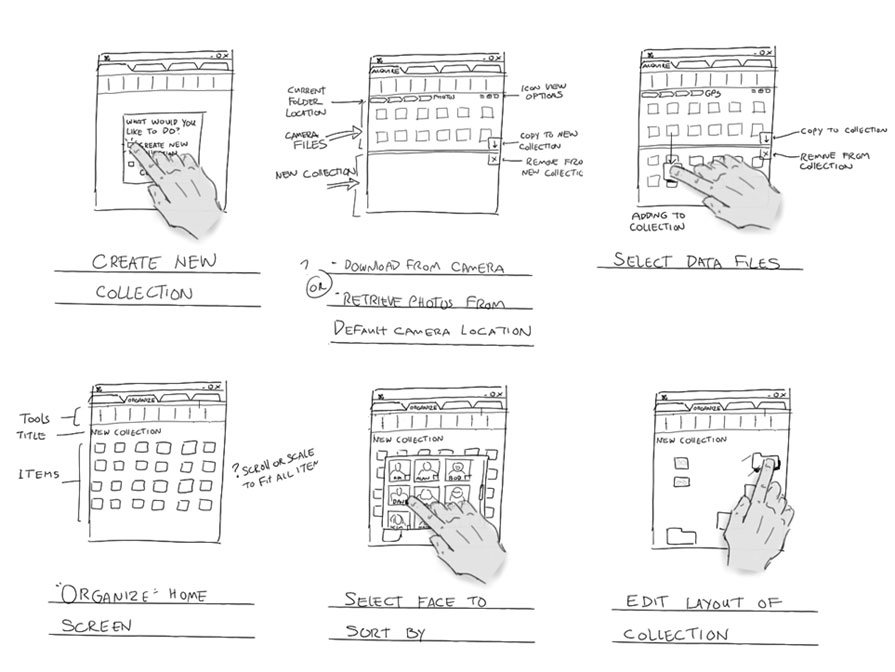
\includegraphics[keepaspectratio,width=\hsize,height=\halfh]
{images/storyboard.jpeg}

\caption[Storyboard Sketching]{
Example of storyboard sketching for drag and drop animation \citep{microsoftStoryboard}.
\imgcredit{Used with permission from Microsoft - Microsoft Copyrighted Content Guidelines}
}
\label{fig:storyboard}
\end{figure}


% Rok Kogovšek
\cleardoublepage
%----------------------------------------------------------------
%
%  File    :  survey-CSS.tex
%
%  Author  :  Rok Kogovšek, TU Graz, Austria
% 
%  Created :  01 Dec 2016
% 
%  Changed :  X Dec 2016
% 
%----------------------------------------------------------------


\chapter{Cascading Style Sheets (CSS)}

\label{chap:CSS}

Knowing the usefulness of animation in web UI and the correct way of animation planing are just the fundemantals for our conceptual plans. Those still need to be implemented to get the end product and here we usually hit a wall build from the various tools, that say they can all solve our problems. Even well established people in the field have stories as such to tell. Val Head actually started with animation due to an interesting Flash workshop. Flash was at that time the de facto king in its era, however as we know, that era is already dead. Nowdays we can acomplish
all we could with Flash and more with just the core parts of the web, namely HTML, CSS and JS
\citep{head2016designing}.

\section{Do Everything You Can With CSS}

\label{sec:everythingCSS}

With Responsive web design (RWD) in our websites and animation being part of the design, see section \ref{sec:anime_dev}, it should be natural to use the guidelines of RWD also in animation planning. \citet{IAWEB} teaches us that one of the RWD guidelines is also Progressive enhancement, which is best described with words of the conceptual authors \citet{champeon2003inclusive}: {\em"Leave no one behind. . . .  accessibility is for everyone, not just the disabled"}. With CSS nowdays being a core part of the web and at the same time being the lowest web component that enables animation with RWD guidelines\footnote{Of course one can just use an animated image, e.q. a GIF with an image sequence, and just append it with HTML into the design. However, this image will become a static component of the design and will not follow RWD guidelines.}, one should always implement with CSS and HTML alone as much of the desired animation as possible. One has only to make sure the browser support for the animated attribute.

Other supporting arguments for use of CSS as the starting point for web UI animation beside responsiveness can be summarized with the the so called "Simple CSS Truths", a list of truths by \citet{palermoCSS} enhanced with the teachings of \citet{IAWEB}:

\begin{description}
\item [CSS allows for separation of concerns] -
 With CSS the form is separated from the page's HTML structure and content. Makes it easier to read, maintain and crawl the code.

\item [CSS has a captive audience] -
 Support for CSS development is huge. At the same time more and more libraries, tools and frameworks focus on improving and simplifing CSS development. 

\item [CSS is fast] - 
 External CSS speeds up HTML downlaod and loading compared to HTMLs with duplicated inline styles. Compared to JavaScript it also processes transitions and animations faster.

\item [CSS is fault-tolarent] - 
 Browser-unknown enhancements are simply ignored by the browser, while the remainder is still used and displayed.

\item [CSS is everywhere] - 
 Modern browsers embrace CSS and feature support by each can be easily found online.
\end{description}

% section everythingCSS (end)

\section{CSS Animation Declaration} % (fold)
\label{sec:declarationCSS}

As stated in section \ref{sec:anime_motion}, animation is about changing an element's attribute(s) over time. In CSS we can redefine it as a switch between CSS styles for a HTML element that happens gradually over time. It is stated that CSS animation should be done with {\em{}Animation} property(ies) and {\em{}Keyframe} rule(s). This may be the most efficient CSS way to accomplish animation, but CSS animation can also be achieved with {\em{}Transition} property(ies) and {\em{}selector} pattern(s)\citep{w3schoolAnime,w3schoolTrans}.


\subsection{Animation Property and Keframe Rule} % (fold)
\label{sub:CSS_animation_keyframe}

The prefered declaration for animation in CSS is done by setting animation properties to the element, that will change through time. This properties just define to which animation steps or keyframes the element is linked to and how the in-between-keyframe states are interpolated through time. \citet{w3schoolAnime} explains the different properties as follows:

\begin{description}
\item [animation-name:] Here the {\em{}@keyframe} rule name is used to link the rule to the element. Since CSS animation is a set of animation properties and keyframe rules, it is a neccasery property.
\item [animation-duration:] Like-wise to the name, duration of the animation is also a neccasery property, since it defaults to 0. Animation is defined as a change over a time, so with the time duration being zero, of course there is no animation. Actual working values can be either seconds (\#s) or miliseconds (\#ms), that define one cycle of the animation.
\item [animation-timing-function:] Defines the progression curve over time, that defines how the animation is interpolated. The valid values are linear, ease, ease-in, ease-out, ease-in-out, cubic-bezier(x1,y1,x2,y1) and steps(stepSize, start, end). Acording to \citet{head2016designing}, most animators have a hard time imagining the effect of functions that start with ease*. While linear and steps are simple to understand and enough for simple animations, the cubic-bezier function should be used, since it can define any desirable curve. The way the cubic-bezier function works, can be observed in figure \ref{fig:curve}.
\item [animation-delay:] Defines how many seconds or miliseconds should the animation start be delayed. The default value is 0. It is useful, when we want multiple elements be animated one after another.
\item [animation-iteration-count:] We can define with a number, how many loops of the cycle should be done or set it to infinite cycles for a non-stop replay. The default value is 1.
\item [animation-direction:] With this property we describe in which way the animation is interpolated and what happens after the 1st cycle of animation. By setting it to the default normal, set it to reset the element into the state before animation and start it again. Reverse always starts from the end keyframe and goes towaqrds the starting keyframe, while alternate will alternate between normal and reverse by the oddness of the cycle number. Another option is the self-explanatory alternate-reverse.
\item [animation-fill-mode:] Defines what happens to an unplayed element, be it after finishing the animation or during a delay wait. By the default none the element has the CSS style outside the keyframe rules. Forwards will use the style of the last keyframe, while backwards will use the style of the first keyframe. A special option is both, that uses the styles of both the start and end keyframe.
\item [animation-play-state:] It is mostly a property used for testing and with control triggers. As the property name states it is either paused or running.
\end{description}

Same as with other CSS properties animation properties can be combined into a single property, simply called animation and where the property values follow as stated:

\begin{description}
\item [animation:] name duration timing-function delay iteration-count direction fill-mode play-state;
\end{description}

\begin{figure}[tp]
\centering
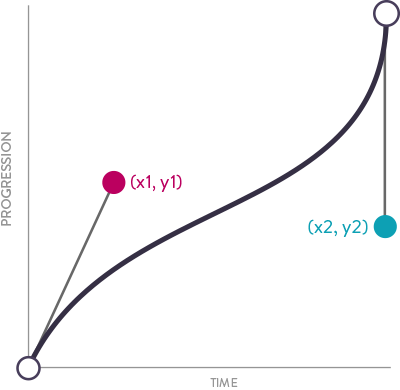
\includegraphics[keepaspectratio,width=\hsize,height=\halfh]
{images/cubicBezier.png}

\caption[Cubic-bezier Function]{
With coordinates for the location of the start and end weight we can define the desired function curve for progression through time by how much each half of the function should be deformed away from a linear function \citep{head2016designing}.
\imgcredit{The image is from the book
"Designing interface animation" by \citet{head2016designing}, used under CC BY 2.0 / It is accessible at {\em{}https://www.flickr.com/photos/rosenfeldmedia/albums/72157671107313626}.
}}
\label{fig:curve}
\end{figure}

While the animation properties just link the element to the desired changes, the actual CSS changes are defined in the @keyframes rule. In the rule we can set the keyframes, that are the finishing times, when a change should end. The keyframe times are simply described with percantage from 0\% as the start keframe and 100\% as the end keyframe. To this times we simply set, which styles should be used at the appointed time. The interpolation function set in with animation property will during proccessing interpolate the undefined percantages. For a better understanding see listing \ref{list:nonmotionAnime}.


\begin{lstlisting}[
language=CSS,
label=list:BibACMIEEE,
caption={[Example of non-motion animation in CSS]%
Simple example of non-motion animation with animation property and keyframes rule. A working example can be found in code/nonmotionAnimationCSS.html.
}
]
div{
	animation: desiredName 4s linear 0s infinite alternate;
}

@keyframes desiredName {
	0%   {background-color:red;opacity: 1;transform: scale(1);}
	25%  {background-color:yellow;transform: scale(0.8);}
	50%  {background-color:blue;transform: scale(1);}
	75%  {background-color:green;transform: scale(1.5);}
	100% {background-color:red;opacity: 0.2;transform: scale(2);}
}
\end{lstlisting}
\label{list:nonmotionAnime}
% subsection CSS_animation_keyframe (end)

\subsection{Transition Property and Selector Pattern} % (fold)
\label{sub:CSS_transition}

\TODO{edit}

\begin{description}
\item [transition-property:] propertyName | all
\item [transition-duration:] 5s
\item [transition-timing-function:] linear | ease | ease-in | ease-out | ease-in-out | cubic-bezier(x1,y1,x2,y1)
\item [transition-delay:] 2s
\end{description}


\begin{lstlisting}[
language=CSS,
label=list:BibACMIEEE,
caption={[Example of non-motion transition in CSS]%
Simple example of non-motion animation with transition property and hover selector. A working example can be found in code/nonmotionTransitionCSS.html.
}
]
div{
	background-color: red;
	opacity: 1;
	transition: all 4s;
}
div:hover{
	background-color:green;
	opacity: 0.2;
	transform: scale(2);
}
\end{lstlisting}

% subsection CSS_transition (end)

% section declarationCSS (end)

\section{CSS Examples} % (fold)
\label{sec:CSS_Examples}

% section CSS_Examples (end)

\subsection{Navigation Animation} % (fold)
\label{sub:navigationCSS}

As stated in \TODO{ref section useful}, animation can help with navigation through tha page. In the examples we show two typical cases of such usage.

\TODO{\subsubsection{Hamburger Icon}} % (fold)
\label{subsub:hamburger}

\citet{vtldesign}
\citep{vtldesign}

\begin{figure}[tp]
\centering

\includegraphics[keepaspectratio,scale=0.5]{images/hamburgerVar.png}

\includegraphics[keepaspectratio,scale=0.5]{images/hamburgerMenu.png}

\caption[Hamburger Examples]{
One the left we have a screenshot of code example hamburgerVariationCSS.html, which shows some of the different ways how hamburger icons are animated. On the right side we have hamburgerMenuCSS.html, that demonstrates the showing and hiding of the menu by hovering over the hamburger icon.
\imgcredit{Screenshot taken by the authors of this survey. The code behind the pages is by using the \cite{hamburgerMenu,hamburgerVar} online snipets as a base.}
}
\label{fig:hamburger}
\end{figure}



\TODO{\subsubsection{Current menu position indicator}} % (fold)
\label{subsub:menu}

% subsection navigationCSS (end)

\subsection{Loading Animation} % (fold)
\label{sub:loadingCSS}

Another use of animation is user feedback, see \TODO{ref section useful}.

\TODO{\subsubsection{Rotating Icon}} % (fold)
\label{subsub:rotation_loader}
2D and 3D

\TODO{\subsubsection{Horizontal movement}} % (fold)
\label{subsub:menu}

dots, progress bar, pulz (wave motion)

% section loadingCSS (end)

% Alexei Kruglov
%----------------------------------------------------------------
%
%  File    :  survey-SVG.tex
%
%  Author  : Alexei Kruglov, TU Graz, Austria
% 
%  Created :  01 Dec 2016
% 
%  Changed :  06 Dec 2016
% 
%----------------------------------------------------------------


\section{Scalable Vector Graphics (SVG)}
\label{sect:SVG}
SVG (Scalable Vector Graphics) is an XML (Extensible Markup Language) based specification for describing two-dimensional graphics in a vector form. It is specified by W3C (World Wide Web Consortium). Initial release was made in 2001, and the latest release (1.1) was in 2011. Currently it is used in all latest major web browsers, such as Google Chrome, Mozilla Firefox and Internet Explorer, and in some vector graphics software editors, as Inkscape and Adobe Illustrator. In contrast to raster images, vector images are resolution independent, as the format itself is lossless. As mentioned before, the graphic is described in an XML textual file, which can be compressed with gzip. As a result of compression, web pages, where SVG is used load faster than those which use standard JPEG or PNG graphics solutions. Because graphics can be directly embedded into HTML, no extra HTTP requests are necessary. Above approaches lead to saving of the bandwidth, which is extremely important on the pages with higher loads. SVG has a support for different graphics effects and animations, which can be further enhanced with CSS and JavaScript. In case SVG graphic is made in a very complex node structure, browser can have problems rendering the image. In this case other technologies can be used. SVG integrates with other W3C standards such as the DOM and XSL. Since the graphics are described in vectors, we can change the properties of those through time to achieve much more complex animation than with just HTML elements \citep{w3schoolSVG}. 

\subsection{Defining Graphical Elementsin SVG} % (fold)
\label{sub:SVG_basic_elemnts}
As mentioned before SVG graphics can be embedded directly into HTML pages as an HTML element:

\begin{lstlisting}[
language=CSS,
label=list:BibACMIEEE,
caption={[Example of SVG Embedded Directyl into HTML]%
Simple example code one circle embedded directyl into HTML.
}
]
<html>
	<body>
		<svg width="100" height="100">
		  <circle cx="50" cy="50" r="40" stroke="green" stroke-width="4" fill="yellow" />
		</svg>
	</body>
</html>

\end{lstlisting}
\label{list:SVGHTML}
\begin{figure}[h]
\centering
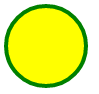
\includegraphics[keepaspectratio,scale=0.5]{images/circle.png}

\caption[SVG Basic Graphical Element]{
This example shows how simple to add one element (circle) embedded directyl into HTML. 
\imgcredit{Screenshot taken by the authors of this survey. The code behind the pages is by using the \citet{CircleHtml} online snippets as a base.}

}
\label{fig:circleHTML}
\end{figure}
SVG consists of different basic graphical elements, from which more complex elements can be derived. Basic elements included in SVG are:
\begin{description}
\item [<rect>]  is used to draw a rectangle and variations of the shape of a rectangle.
\item [<circle>] creates a simple circle with color options.
\item [<line>] draws a line.
\item [<polygon>] is used to create a graphic that contains at least three sides.
\item [<polyline>] provides any shape consisting of straight lines.
\item [<path>] defines a path. Use of a SVG editor is strongly encourage for path drawing to create complex graphics.
\end{description}

With these simple basic elements, one can build very complex shapes. With heli one has also additional graphics functions, where creation of a moving figure is also included. However, if these figures are created just by using SVG, the program code will be very large and difficult to read.
\begin{figure}[h]
\centering
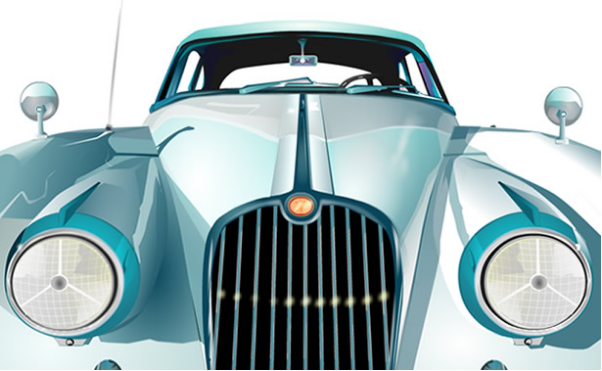
\includegraphics[keepaspectratio,scale=0.5]{images/Car_svg.png}

\caption[Complex Image with Simple SVG Elements]{
Example to create one complex picture with simple SVG elements, with help geomety and color options.
\imgcredit{Screenshot taken by the authors of this survey. The code behind the pages is by using the \citet{CarSVG} online snippets as a base.}

}
\label{fig:Circle_HTML}
\end{figure}
% SVG basic graphical elements (end)
\subsection{Using SVG in CSS Animation } % (fold)
\label{sub:usingSVGanime}
SVG element is a specific DOM element, which includes himself syntax standard HTML-element. SVG elements have unique tags, attributes and behaviors that enable them to determine any form that offer the opportunity to essentially produce directly to the DOM, images, and thereby benefit from the JavaScript and CSS-based manipulation. There are three main advantages to create graphics in SVG comaped to statc images:
\begin{enumerate}
\item SVG can be compressed incredibly well. Certain images as SVGs are smaller than their PNG / JPEG equivalents.
\item SVG graphics can be scaled without any loss of clarity to any resolution. Therefore they look sharp on all desktop and mobile screens.
\item One can animate the individual components of the SVG graphic's performance with CSS or/and JavaScript. Keep in mind that SVG elements take some of the standard CSS properties, but not all.
\end{enumerate}

 In addition, SVG takes a certain set of "presentation" attributes, such as fill, x and y, which also serve to determine how the SVG is visually observed. There is no functional difference between the SVG specification of style using CSS, or as an SVG attribute \citep{w3schoolSVG}. In short, to animate and SVG, one has to:
\begin{enumerate}
\item Define the imeage as vectors in SVG.
\item Tranform the vectors with SVG, CSS or JavaScript.
\end{enumerate}
\begin{lstlisting}[
language=CSS,
label=list:BibACMIEEE,
caption={[SVG Declaration Example for Animation]%
SVG declaration example for animation.
}
]
<animateTransform attributeName="transform"
		attributeType="XML"
		type="translate"
		values="0 50;0 -50;"
		dur="2s"
		repeatCount="indefinite"/>

\end{lstlisting}
\label{list:animateTransorm}
%\subsubsection {Create SVG stucture into HTML} % (fold)


\begin{figure}[h]
\centering

\includegraphics[keepaspectratio,scale=0.5]{images/icon_svg.png}

\includegraphics[keepaspectratio,scale=0.5]{images/beer_svg.png}

\caption[SVG Animation Examples]{
Left example SVG is created by the authors to achieve a a trash bin animation with CSS. While the right example is a pure SVG beer animation. 
\imgcredit{Screenshots taken by the authors of this survey. The animation code behind the trash bin is done by the authors, while the SVG objects are provided by \citet{trashSVG}.The beer code is based on the \citet{beerSVG} online snippets as a base.}

}
\label{fig:SVGExamples}
\end{figure}


\begin{lstlisting}[
language=CSS,
label=list:BibACMIEEE,
caption={[Create SVG Stucture into HTML]%
The definition of the trash bin vectors, in figure \ref{fig:SVGExamples}, with the path element, proveded by \citet{trashSVG}.
}
]
<svg class="svg-icon" viewBox="0 0 20 20">
		<path id="svg-doc" d="M15.475,6.692l-4.084-4.083C11.32,
		2.538,11.223,2.5,11.125,2.5h-6c-0.413,0-0.75,0.337-0.75,
		0.75v13.5c0,0.412,0.337,0.75,0.75,0.75h9.75c0.412,
		0,0.75-0.338,0.75-0.75V6.94C15.609,6.839,15.554,6.771,
		15.475,6.692 M11.5,3.779l2.843,2.846H11.5V3.779z
		M14.875,16.75h-9.75V3.25h5.625V7c0,0.206,0.168,0.375,
		0.375,0.375h3.75V16.75z"
		transform="scale(0.25) translate(27.5)"></path>

		<path id="svg-bottom" fill="none" d="M16.471,
		5.962c-0.365-0.066-0.709,0.176-0.774,0.538l-1.843,
		10.217H6.096L4.255,6.5c-0.066-0.362-0.42-0.603-0.775-0.538
		C3.117,6.027,2.876,6.375,2.942,6.737l1.94,10.765c0.058,
		0.318,0.334,0.549,0.657,0.549h8.872c0.323,0,0.6-0.23,
		0.656-0.549l1.941-10.765C17.074,6.375,16.833,6.027,16.471,
		5.962z"
		transform="scale(0.75) translate(4,20)"></path>

		<path id="svg-deck" fill="none" d="M16.594,3.804H3.406
		c-0.369,0-0.667,0.298-0.667,0.667s0.299,0.667,0.667,
		0.667h13.188c0.369,0,0.667-0.298,0.667-0.667S16.963,
		3.804,16.594,3.804zM9.25,3.284h1.501c0.368,0,0.667-0.298,
		0.667-0.667c0-0.369-0.299-0.667-0.667-0.667H9.25c-0.369,
		0-0.667,0.298-0.667,0.667C8.583,2.985,8.882,3.284,9.25,3.284z"
		transform="scale(0.75) translate(4,20)"></path>
	</svg>

\end{lstlisting}
\label{list:SVGStuctureHTML}

% \subsubsection {Define keyframe in CSS} % (fold)
\begin{lstlisting}[
language=CSS,
label=list:BibACMIEEE,
caption={[SVG Animation with CSS Declaration]%
The animation of the trash bin vectors, in figure \ref{fig:SVGExamples}, with the path element, proveded by \citet{trashSVG}. The animation wokrs together with the vectors in the previous listing.
}
]
#svg-doc{
	fill:red;
	animation: doc-delete 4s linear infinite;
}

#svg-deck{
	transform-origin: 100% 50%;
	animation: deck-rot 4s linear infinite;
}

@keyframes doc-delete {
	0% { transform: translate(75%) scale(0.25); }
	15% { transform: translate(75%) scale(0.25); }
	65% { transform: translate(85%,150%) scale(0.1) rotate(-180deg);}
	100% { transform: translate(85%,150%) scale(0.1); opacity: 0;}
}

@keyframes deck-rot {
	0% { transform: translate(-9%, 440%) rotate(0deg) scale(0.75); }
	25% { transform: translate(-9%, 440%) rotate(90deg) scale(0.75);}
	40% { transform: translate(-9%, 440%) rotate(90deg) scale(0.75);}
	65% { transform: translate(-9%, 440%) rotate(0deg) scale(0.75);}
	100% { transform: translate(-9%, 440%) rotate(0deg) scale(0.75);}

\end{lstlisting}
\label{list:Keys_CSS}

% Helmut Zöhrer
\cleardoublepage
%----------------------------------------------------------------
%
%  File    :  survey-JS.tex
%
%  Author  :  Helmut Zöhrer, TU Graz, Austria
% 
%  Created :  01 Dec 2016
% 
%  Changed :  X Dec 2016
% 
%----------------------------------------------------------------


\chapter{JavaScript (JS)}

\label{chap:JS}

\TODO{CHAPTER INTRO IS MISSING - check chapter 2 and 3}

\section{When to Use JS instead of CSS}

As a rule of thumb, JS should not be used if the same effect could be achieved with plain CSS. This is due to performance and resource management reasons. Just when CSS is stretched to its limits, JS should be used. There is a rough distinction whether to use CSS or JS for particular kinds of tasks:
\begin{itemize}
	\item Use CSS animations for simple transitions, like changing the state of a UI element.
	\item Use JS animations to get advanced effects like bouncing, stop, pause, rewind, or slow down (there is more control over animations).
	\item When choosing to animate with JS, considering using the Web Animations API or a modern framework (comfortable to work with) may be desirable.
	\item Using both CSS and JS works also well:
	\begin{itemize}
		\item perform animations with CSS
		\item control states with JS
	\end{itemize}
\end{itemize}


\section{Examples of Useful Animations with JS}

\TODO{this!}
\TODO{citing with: \citet{googleDev} or \citep{googleDev}}


\begin{lstlisting}[
language=JavaScript,
label=list:BibACMIEEE,
caption={[Some Code Snippet]%
This is a code snippet where JS is used in a meaningful way.
}
]
// create some nodes
var headline = document.createElement('h1');
var text = document.createTextNode('Dies ist eine Überschrift');
// "offline" node manipulation
headline.appendChild(text);
// adding node to DOM
document.getElementsByTagName("body")[0].appendChild(headline);
\end{lstlisting}

\cleardoublepage
%----------------------------------------------------------------
%
%  File    :  survey-concl.tex
%
%  Author  :  Keith Andrews, IICM, TU Graz, Austria
% 
%  Created :  27 May 1993
% 
%  Changed :  16 Nov 2010
% 
%----------------------------------------------------------------


\chapter{Concluding Remarks}

\label{chap:Concl}

Through the course of further investigating web animations, we realized that animations are not merely there to make a website appear more beautiful, but to carry meaning as well. So, if a user sees a hamburger icon, they should / and nowadays probably do know what this icon stands for. 

Numerous examples of coding 


\cleardoublepage
\printbibliography[heading=bibintoc]


\end{document}